\section{Indekser}
\subsection*{Hvorfor indekser?}
\begin{frame}{Indekser}
    \begin{itemize}[<+->]
        \item Rows er ikke sortert
        \item $\rightarrow$ finne informasjoner med WHERE tar tid
        \item Indekser er ekstrastrukturer som forenkler søking i tabeller
        \item Kan være en eller flere kolonner 
        \item Indekser funker som ordbok/lookup table
        \item Ulempe: De tar plass, må oppdateres
        \item Primærnøkler har automatisk en indeks på seg
        \item To typer indekser:
            \begin{itemize}
                \item B-trær
                \item Hashing
            \end{itemize}
    \end{itemize}
\end{frame}

\subsection*{B-trær}
\begin{frame}{B-trær}
    \begin{columns}
    \begin{column}{0.48\textwidth}
    \begin{figure}
        %\centering
        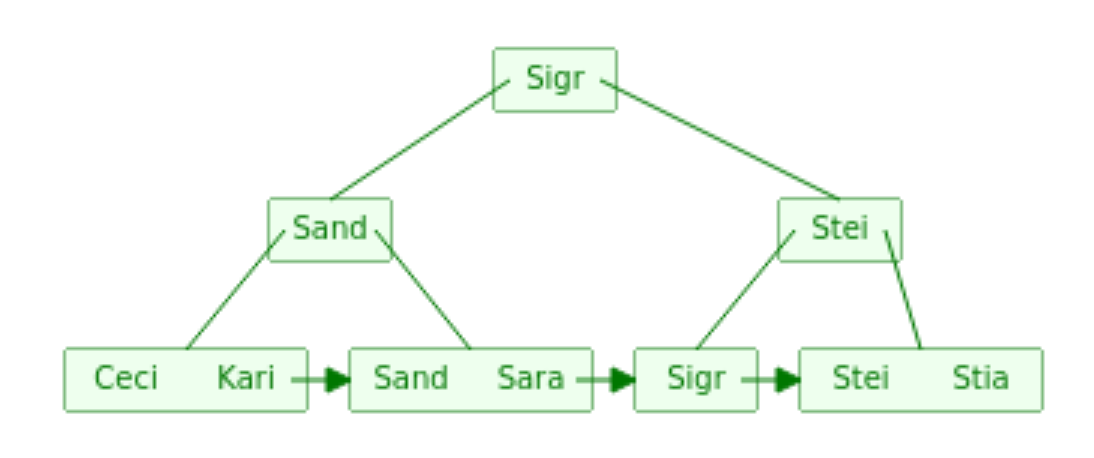
\includegraphics[height = 2.9cm]{images/btre.png}
        \caption{Eksempel B-tre}
        \label{fig:btree}
    \end{figure}
    \end{column}
    \begin{column}{0.48\textwidth}
    \begin{itemize}[<+->]
        \item Data er organisert som et søketre
        \item Alle elementer er leaves i treet 
        \item Leaves er sortert
        \item Leting etter elementer skjer gjennom graftraversal
        \item Hvis element er mindre, gå til venstre
        \item Hvis element er større, gå til høyre
        \item Kjøretiden blir $O(log(n))$ istedenfor $O(n)$
    \end{itemize}
    \end{column}
    \end{columns}
\end{frame}

\subsection*{Hashing}
\begin{frame}{Hashing}
    \begin{columns}
    \begin{column}{0.48\textwidth}
    \begin{figure}
        %\centering
        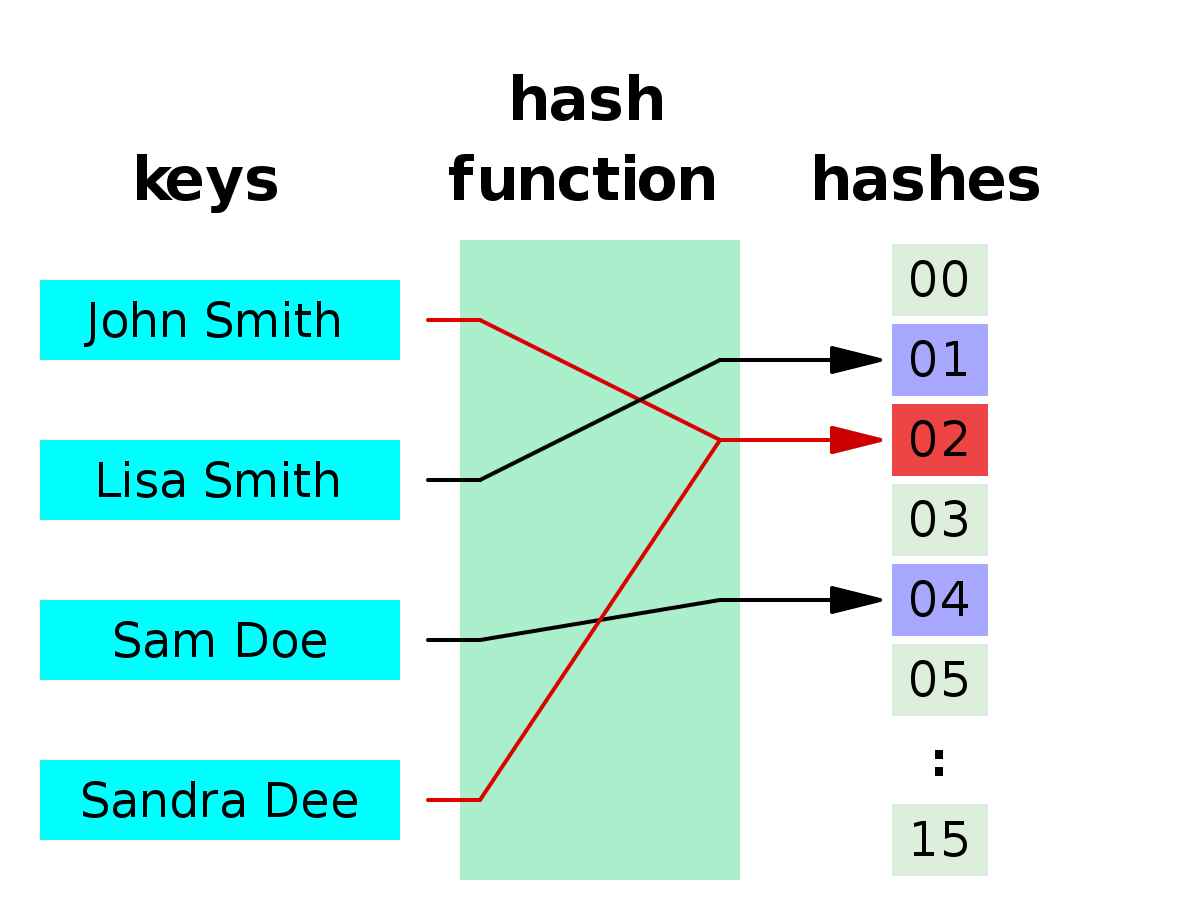
\includegraphics[height = 3.8cm]{images/hashing.png}
        \caption{Eksempel Hashing}
        \label{fig:hashing}
    \end{figure}
    \end{column}
    \begin{column}{0.48\textwidth}
    \begin{itemize}[<+->]
        \item Data blir komprimert med en engangsfunksjon
        \item Data blir lagt som liste av hashes
        \item Listen kan ikke sorteres
        \item Listeinnholdet følger ingen pattern
        \item Kjøretiden blir $O(1)$ istedenfor $O(n)$
        \item Range-Selection er drittslangsom
    \end{itemize}
    \end{column}
    \end{columns}
\end{frame}

\subsection*{Eksempel}
\begin{frame}{Hvilke indekser skulle man ha?}
    \begin{itemize}[<+->]
        \item Students(Student number*, First Name, Last Name, Gender)
        \item Indekser: Last Name,(First Name, Last Name)
        \item Staff(Staff number*, First Name, Last Name, Position)
        \item Indekser: Last Name,(First Name, Last Name), Position
        \item Course(Course Code*, Course Name, Credits)
        \item Indekser: Name? Credits?
        \item Study(Study Code*, Study name)
        \item Indekser: Study name
        \item StudyDesign(Study Code*, Course Code*, Semester Number)
        \item Indekser: Semester Number
        \item Results(Serial number*, Student number*, Grade)
        \item Indekser: Ingen?
    \end{itemize}
\end{frame}

\subsection*{Spørretid}
\begin{frame}{Spørsmål?}
    \begin{figure}
        \centering
        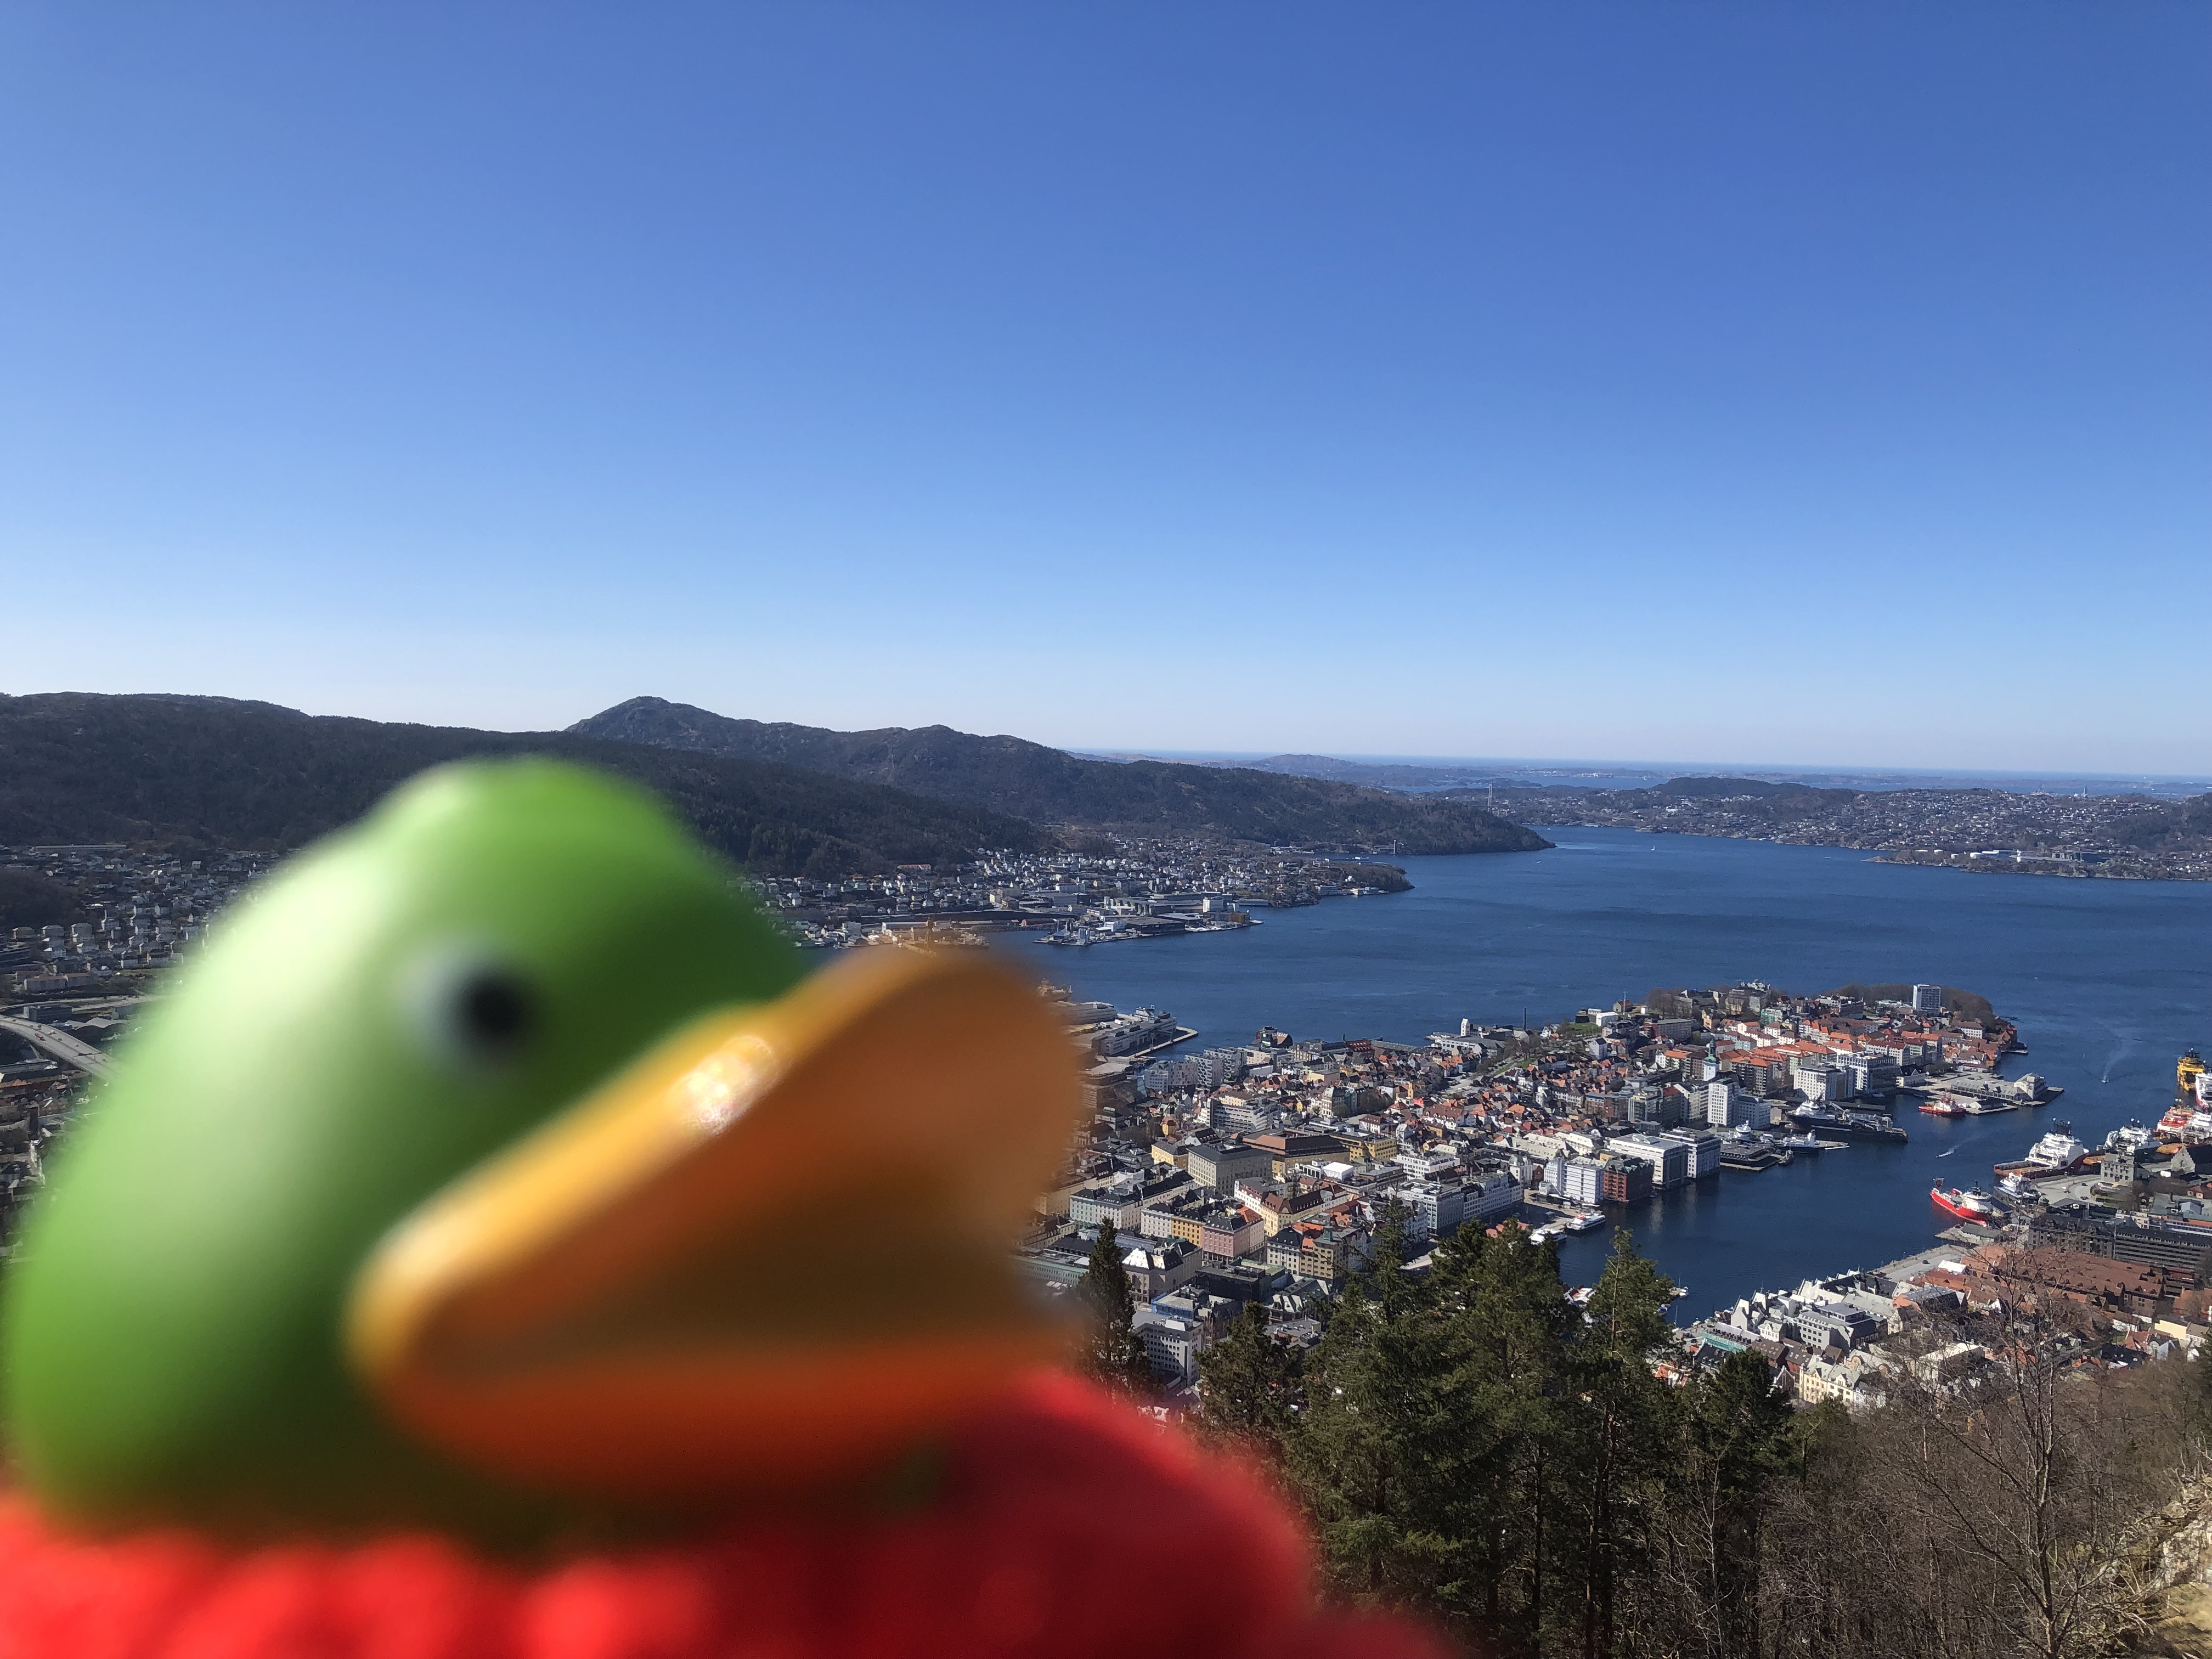
\includegraphics[height = 4.9cm]{images/guillaume10.jpg}
        \caption{Guillaume på Fløyen}
        \label{fig:guillaume10}
    \end{figure}
\end{frame}
